%#
%# Lab study
%# https://github.com/IIS-Lab/ShibatoM/wiki/Analysis-of-lab-study をまとめる.
%############################

\chapter{RealCodeが出題する演習問題の分類評価}
\label{section:lab-study}
\graphicspath{{Chapters_evaluation/Figs/}}


\ref{section:ta_evaluation},\ref{section:interview-study}章にて述べた評価実験により,イシューをプログラミング演習問題へと転用する事で,既存の学習環境にはない独自のプログラミング演習問題を提供可能である事が明らかとなった.
しかし,RealCodeの演習問題から何を学べるのかは明らかとなっていない.
そこで我々は,RealCodeから何を学べるのかを理解するために,著者によるRealCodeの演習問題の評価を行った.
本章では,この評価実験の詳細と結果について述べる.


\section{実験方法}

\begin{figure}[t]
	\centering
  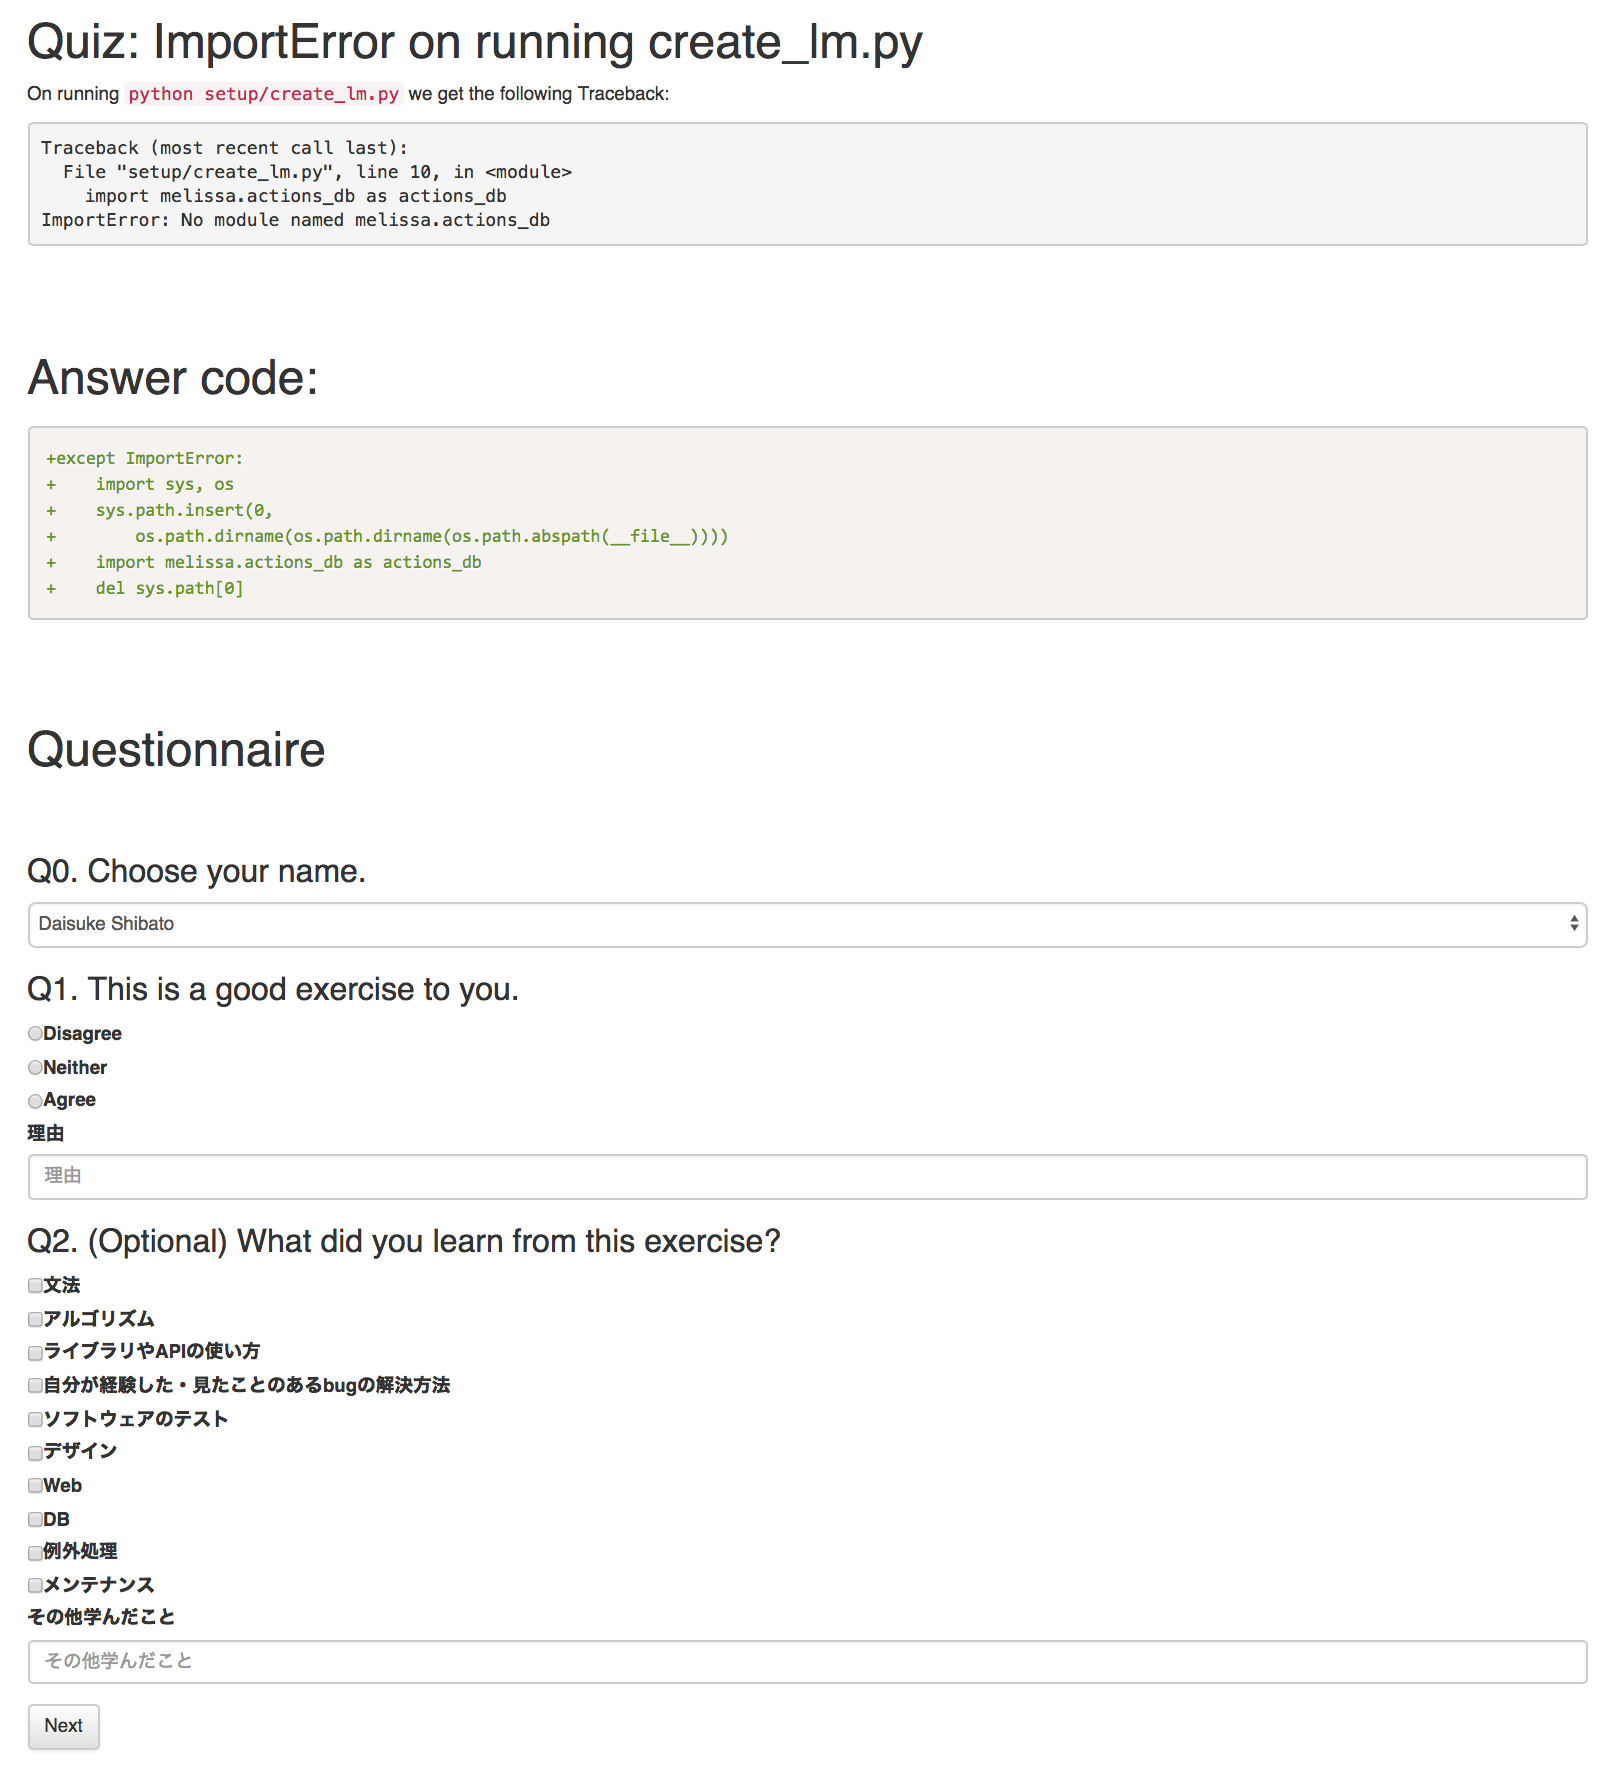
\includegraphics[width=1.0\columnwidth]{20181218-lab-study-interface-all.png}
  \caption{評価に用いたインターフェース.}
  \label{fig:lab-study}
\end{figure}

現在のRealCodeのプロトタイプに存在する \xxx 件の演習問題に対し,著者は以下の質問に5段階で評価を行った(1: 全く同意しない -- 5: 強く同意する).

\begin{itemize}
  \item[Q1.] Is this a good exercise to you?
  \item[Q2.] 学べることは?
  \begin{itemize}
  	  \item Q2-1. 教科書で全く扱われていない範囲である
   	  \item Q2-2. 新しいAPIやライブラリの知識を必要とする
      \item Q2-3. あまり知られていないバグの修正を題材にしている
      \item Q2-4. 本番環境におけるバグの影響を実感できる
      \item Q2-5. ソフトウェアを本番稼働するための知識を必要とする
      \item Q2-6. チーム開発を意識したコードの書き方
  \end{itemize}
\end{itemize}



\section{実験結果}








